\subsection{Drag perturbation}
In this section, there is simplifying the assumption that drag force is in the S direction.
$$
F_{drag} = \dfrac{1}{2}\rho v^2 s C_D \to \boldsymbol{\mathrm{F_{drag}}} = -\dfrac{1}{2}\rho v^2 s C_D \vec{S}
$$
$$
\boldsymbol{\mathrm{a_{drag}}} = -\dfrac{1}{2m_s}\rho v^2 s C_D \vec{S}
$$
From \eqref{eq:all_perturbation_equations} we know the effect of other forces on orbital elements. Here is the result of perturbation forces on orbital elements.
The simulation has been in the Jupyter notebook. the results are presented here.

\begin{figure}[H]
    \centering
    \includegraphics[width=0.85\textwidth]{../Figure/Q2/orbital_elements_drag_100.pdf}
    \caption{Variation of Parameter due to drag perturbation for 100 seconds}
\end{figure}

\begin{figure}[H]
    \centering
    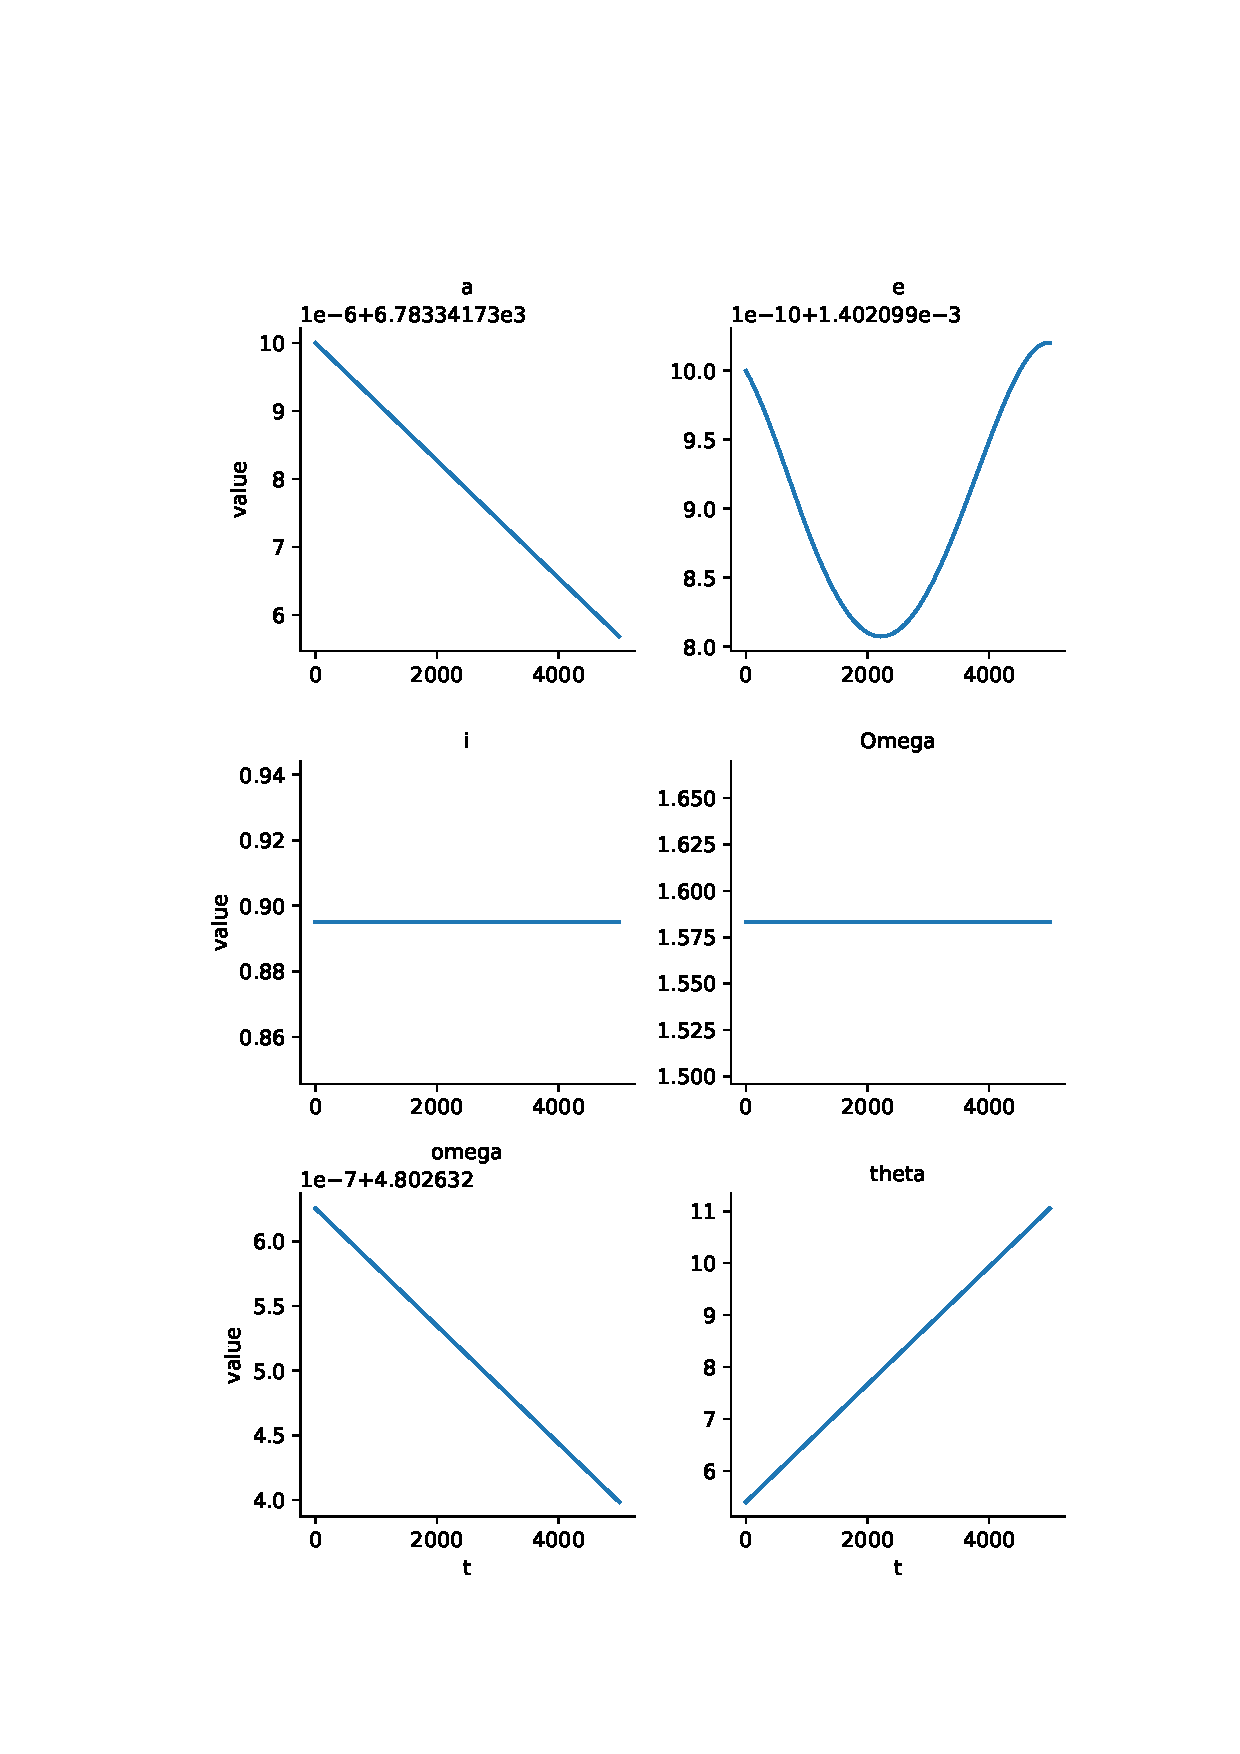
\includegraphics[width=0.85\textwidth]{../Figure/Q2/orbital_elements_drag_5000.pdf}
    \caption{Variation of Parameter due to drag perturbation for 5000 seconds}
\end{figure}

\begin{figure}[H]
    \centering
    \includegraphics[width=0.85\textwidth]{../Figure/Q2/orbital_elements_drag_10000.pdf}
    \caption{Variation of Parameter due to drag perturbation for 10000 seconds}
\end{figure}